\documentclass[12pt]{report}
% Set page margins
\usepackage[margin=4cm]{geometry}

\usepackage[]{graphicx}
\usepackage{setspace}
\usepackage{amsmath}
\usepackage{amsthm} % theorems, examples, definitions
\usepackage{commath} % norm
\usepackage{amssymb}
\usepackage{nicematrix}
\singlespace % interlinea singola

\usepackage{hyperref}
\hypersetup{
	colorlinks=true,
	linkcolor=blue,
	filecolor=magenta,
	urlcolor=blue,
}
 
% All page numbers positioned at the bottom of the page
\usepackage{fancyhdr}
\fancyhf{} % clear all header and footers
\fancyfoot[C]{\thepage}
\renewcommand{\headrulewidth}{0pt} % remove the header rule
\pagestyle{fancy}

% Changes the style of chapter headings
\usepackage{titlesec}

\titleformat{\chapter}
   {\normalfont\LARGE\bfseries}{\thechapter.}{1em}{}

% Change distance between chapter header and text
\titlespacing{\chapter}{0pt}{35pt}{\baselineskip}
\usepackage{titlesec}
\titleformat{\section}
	[hang] % \textlessshape\textgreater
	{\normalfont\bfseries\Large} % \textlessformat\textgreater
	{} % \textlesslabel\textgreater
	{0pt} % \textlesssep\textgreater
	{} % \textlessbefore code\textgreater
\renewcommand{\thesection}{} % Remove section references...
\renewcommand{\thesection}{\arabic{section}} %... from sections
\usepackage{titlesec}

\setcounter{tocdepth}{5}
\setcounter{secnumdepth}{5}

% Prevents LaTeX from filling out a page to the bottom
\raggedbottom

\usepackage{tabularx}
\usepackage{booktabs}
\usepackage{color}
\usepackage{xcolor}
\usepackage{enumitem}
\usepackage{amsmath}
\usepackage{subcaption}
\usepackage{physics}
\usepackage{minted}

\theoremstyle{definition}
\newtheorem{definition}{Definition}[section]
\theoremstyle{definition}
\newtheorem{example}{Example}[section]
\newtheorem{theorem}{Theorem}[section]
\newtheorem{corollary}{Corollary}[theorem]
\newtheorem{lemma}[theorem]{Lemma}
\newtheorem*{remark}{Remark}
\newcommand{\iu}{\mathrm{i}\mkern1mu}

\newcommand\scalemath[2]{\scalebox{#1}{\mbox{\ensuremath{\displaystyle #2}}}}

\makeatletter
\@ifpackageloaded{hyperref}%
  {\newcommand{\mylabel}[2]% #1=name, #2 = contents
	{\protected@write\@auxout{}{\string\newlabel{#1}{{#2}{\thepage}%
	  {\@currentlabelname}{\@currentHref}{}}}}}%
  {\newcommand{\mylabel}[2]% #1=name, #2 = contents
	{\protected@write\@auxout{}{\string\newlabel{#1}{{#2}{\thepage}}}}}
\makeatother

\makeatletter
\let\original@algocf@latexcaption\algocf@latexcaption
\long\def\algocf@latexcaption#1[#2]{%
  \@ifundefined{NR@gettitle}{%
	\def\@currentlabelname{#2}%
  }{%
	\NR@gettitle{#2}%
  }%
  \original@algocf@latexcaption{#1}[{#2}]%
}
\makeatother

\newcounter{cases}
\newcounter{subcases}[cases]
\newenvironment{cs}
{
	\setcounter{cases}{0}
	\setcounter{subcases}{0}
	\newcommand{\case}
	{
		\par\indent\stepcounter{cases}\textbf{Case \thecases.}
	}
	\newcommand{\subcase}
	{
		\par\indent\stepcounter{subcases}\textit{Subcase (\thesubcases):}
	}
}
{
	\par
}
\renewcommand*\thecases{\arabic{cases}}
\renewcommand*\thesubcases{\roman{subcases}}

\begin{document}
\begin{titlepage}
	\clearpage\thispagestyle{empty}
	\centering
	\vspace{1cm}

	\includegraphics[scale=0.58]{../../images/unipi-marchio.eps}

	{\normalsize \noindent Dipartimento di Informatica \\
			Corso di Laurea in Informatica \par}
	
	\vspace{2cm}
	{\huge \textbf{Assignment 01} \par }
	\vspace{1cm}
	{\large Competitive Programming and Contests}

	\vspace{3cm}

	\begin{minipage}[t]{0.47\textwidth}
		{\large{Prof. Rossano Venturini}}
	\end{minipage}\hfill\begin{minipage}[t]{0.47\textwidth}\raggedleft
		{\large {Giacomo Trapani - 600124}}
	\end{minipage}

	\vspace{3cm}

	{\normalsize Academic Year 2024/2025 \par}

	\pagebreak
\end{titlepage}
\paragraph*{Exercise 1}
This exercise requires the implementation of a method to check if a given tree
is a \textbf{binary search tree}, which means that for each node its key K must
be greater than that of its left child and less than that of its
right child. For the purposes of this exercise, a relaxation of this condition is
chosen: duplicates are allowed on one side of the binary search tree.

The idea behind the algorithm implemented is to work with lower and upper bounds. For
each node, we check whether its value lies between the bounds, the values of which depend
on its parent (node).

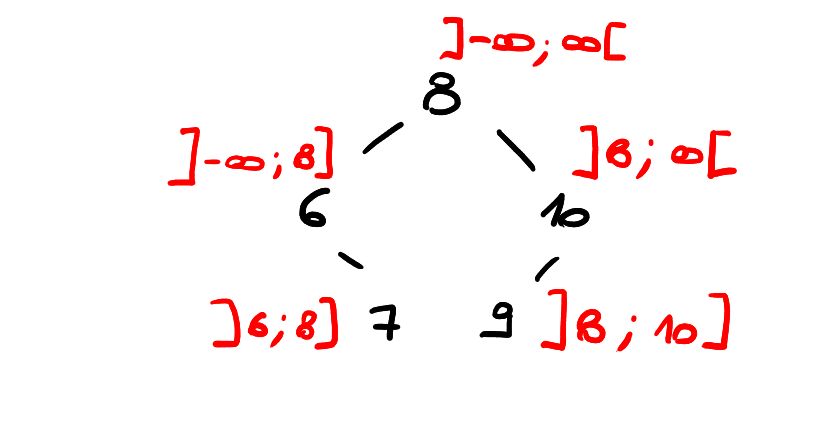
\includegraphics[scale=0.4]{./images/ex1-range-sample.png}


The algorithm implemented takes O(n) time.
\paragraph*{Exercise 2}
This exercise requires the implementation of a method to calculate the maximum path sum
between two leaves in a binary tree. For the purposes of this exercise,
the value \texttt{-i32::MIN} has been chosen to be returned whenever we cannot find a path
between two leaves; also, the implementation of the \texttt{Tree} struct has been changed
to work with \texttt{i32} values as the previous implementation would not have allowed for
negative values.

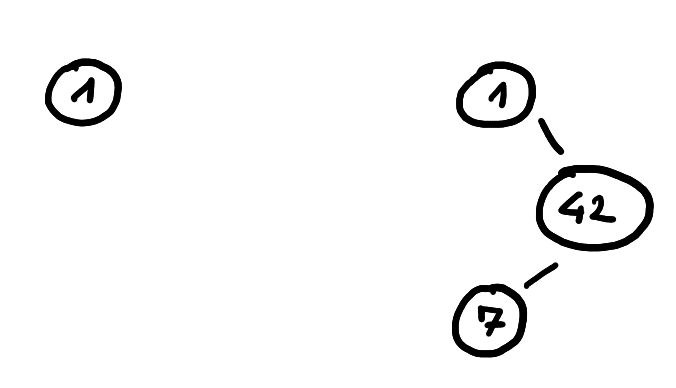
\includegraphics[scale=0.35]{images/ex2-trees-no-mps.png}

\pagebreak
The algorithm implemented measures two different things
(ref. to \linebreak \texttt{rec\_maximum\_path\_sum}):
\begin{itemize}
\item the return value is the maximum path sum for a root-to-leaf path i.e. the maximum
path sum from \texttt{index} to any of the leaves below,
\item the value inside the pointer \texttt{global\_max} is the maximum path sum for a
leaf-to-leaf path i.e. the maximum path sum in the tree rooted in \texttt{index}
between two of the leaves below it.


The algorithm implemented takes O(n) time.
\end{itemize}
\end{document}